\chapter{Biblioteki i narzędzia}
\label{chap:libs}

\section{DirectX 11}

DirectX 11~\cite{DX11Cytat} jest to biblioteka graficzna wykorzystywana głównie do tworzenia gier komputerowych (np. Baldur's Gate 3, Wiedźmin 3) lub innych aplikacji graficznych. Biblioteka została stworzona w 2009 roku przez firmę Microsoft. Dostępna jest tylko na komputerach z systemem Windows i konsolach Xbox.


W silniku wykorzystywana jest do grafiki poprzez shadery. Shader to program działający na karcie graficznej.

\section{Win32}
Win32~\cite{win}, jest to interfejs programistyczny systemu Windows. Zawiera w sobie funkcje umożliwiające działanie programów w systemie. Okno prezentowanego silnika zostało stworzone za pomocą tej biblioteki.

\section{ImGui}

ImGui~\cite{imgui} to biblioteka wykorzystywana do tworzenia interfejsu użytkownika. Napisana jest w myśl paradygmatu "Immediate Mode GUI" (IMGUI), który głównie polega na tym, że interfejs jest cały czas odświeżany, nie przechowuje on stanu między klatkami przez co jest zawsze zsynchronizowany z danymi (inaczej niż w interfejsach tworzonych za pomocą win32, retained mode). Biblioteka ta jest również łatwiejsza w obsłudze niż np. biblioteka Qt. 


ImGui wykorzystuje wybrany backend (w tym przypadku backend napisany w DX11) aby renderować interfejs.

\section{Assimp}

Assimp~\cite{Assimp}-- Open Asset Import Library jest to biblioteka umożliwiająca łatwe ładowanie modeli 3D w różnych formatach. W silniku wykorzystywane są formaty obj, glb. Napisana jest w języku C++. Modele 3D pobrano z internetu, linki dostępne są w pliku ModelCredits.txt, w folderze projektu. 

\section{Stb\_Image}

Stb\_Image~\cite{StbIMG} jest to biblioteka wykorzystywana do ładowania tekstur w różnych formatach. Silnik wykorzystuje format .hdr używany w teksturach otoczenia. Biblioteka napisana jest w języku C. Tekstury pobrano ze strony ,,Poly Haven", jest to darmowa biblioteka tekstur hdr, tekstur pbr (materiały) i modeli 3D.

\section{Visual Studio}

Program napisano wykorzystując IDE (ang. \textit{Integrated development environment}) Visual Studio w wersji Community 2022~\cite{vs2022}. Korzystano z dodatkowych pakietów: ,,Programowanie aplikacji klasycznych w języku C++" i ,,Projektowanie gier przy użyciu języka C++".  Z rozszerzeń wykorzystano ,,HLSL Tools for Visual Studio".

\section{Premake}
Jako narzędzie do konfiguracji projektu korzystano z Premake~\cite{premake}. Premake jest to narzędzie które czytając skrypt, napisany w języku Lua, tworzy plik projektu np. solucje Visual Studio. Do pełnej automatyzacji budowania plików projektów i bibliotek dodatkowo użyto skryptów .bat.

\chapter{Prezentacja silnika}

\section{Interfejs}
%
Interfejs podzielony jest na 4 sekcje:
\begin{itemize}
    \item \textbf{Viewport} -- tutaj renderowany jest obraz.
    \item \textbf{Spheres} -- ustawienia położenia i promienia każdej sfery.
    \item \textbf{Materials} -- ustawienia parametrów materiałów.
    \item \textbf{Settings} -- ustawienia renderowania 
\end{itemize}

\begin{figure}[htbp]
    \centering
    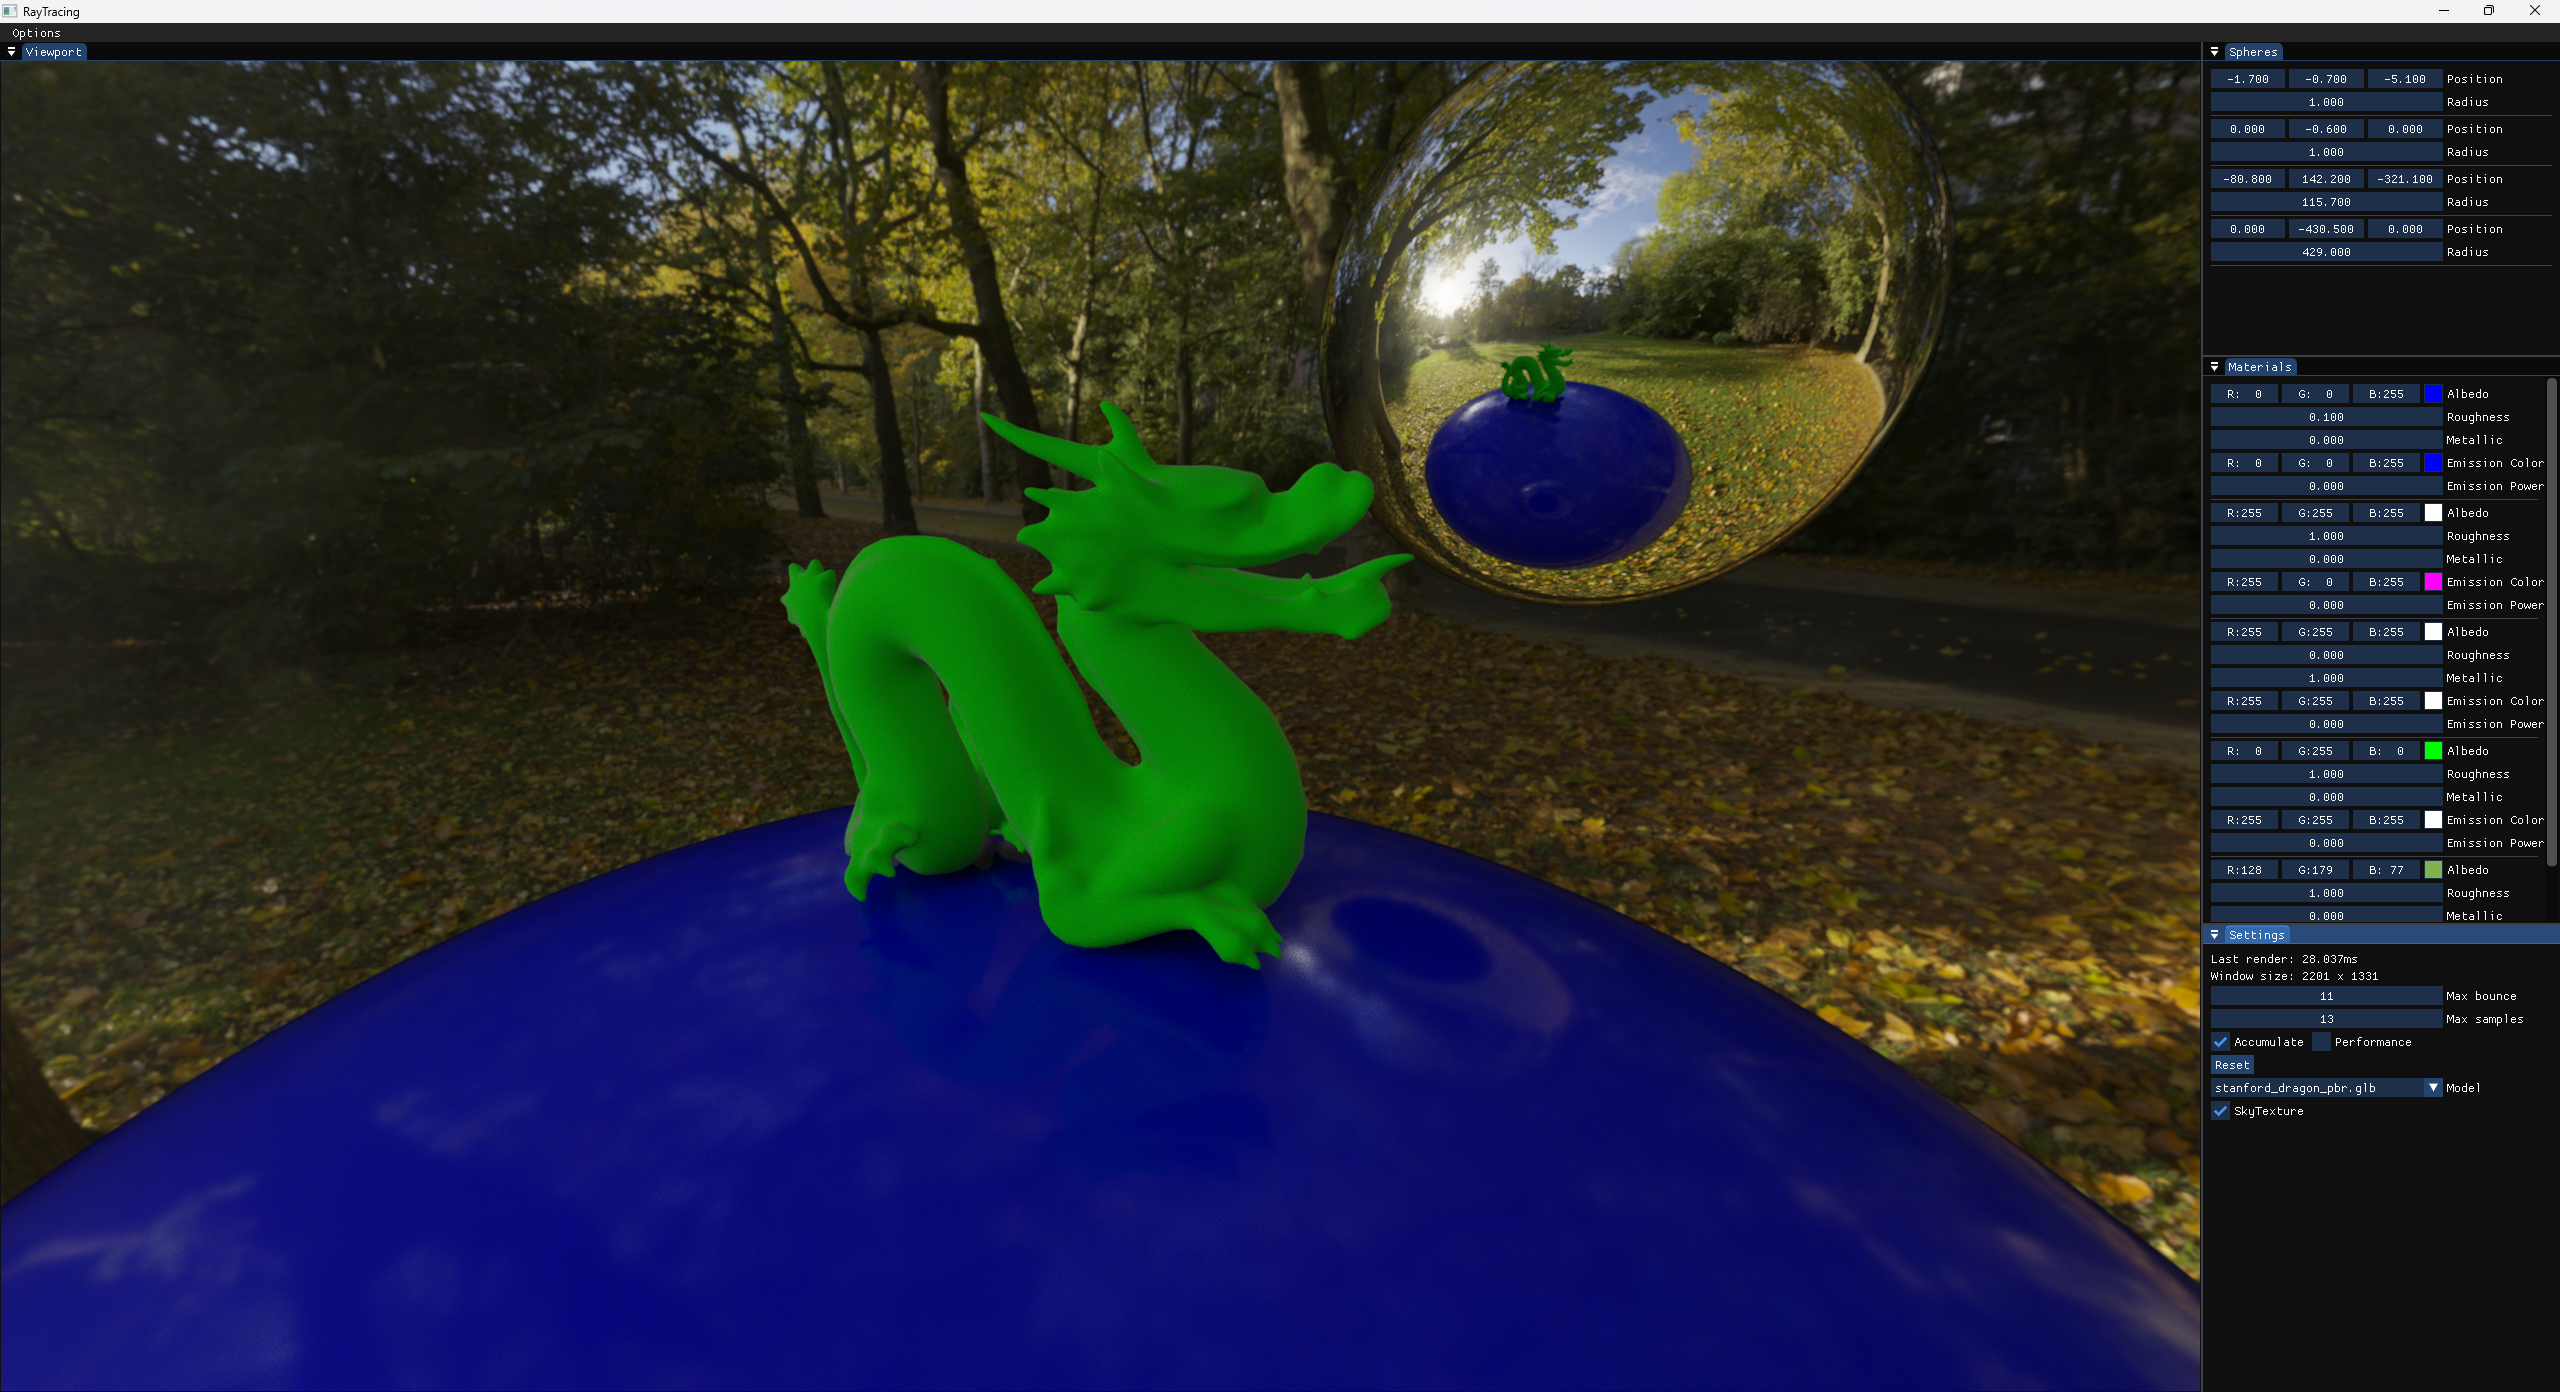
\includegraphics[width=1\textwidth]{Interfejs} 
    \caption{
      Zdjęcie przedstawia interfejs silnika.
      \todo[inline]{Raczej: ,,Interfejs stworzonego w~ramach pracy silnika ray-tracing''}
      \todo[inline]{To nie częścią opisu narzędzi i~technologii}
    }
    \label{fig:interfejs}
\end{figure}

\section{Elementy silnika}

\begin{figure}[H]
    \centering
    \includegraphics[width=1\textwidth]{SchematSilnika} 
    \caption{Schemat silnika.}
    \label{fig:uml}
\end{figure}

\section{Opis potoku graficznego}

Potok graficzny (ang. \textit{graphics pipeline} lub \textit{rendering pipeline}) jest to sekwencja kroków które należy wykonać aby otrzymać obraz na ekranie. Na rysunku \ref{fig:pipeline} widoczny jest cały potok graficzny używany w DX11. Strzałki oznaczają przepływ danych np. vertex shader otrzymuje dane z fazy Input assembler, wykonuje na nich swoje obliczenia i przekazuje dalej do hull shadera. 

\begin{figure}[H]
    \centering
    \includegraphics[width=0.8\textwidth]{RenderingPipeline} 
    \caption{Zdjęcie przedstawia potok graficzny w DirectX 11. \cite{dx11}}
    \label{fig:pipeline}
\end{figure}

Najważniejszymi shaderami w potoku są vertex shader i pixel shader (pixel shader czasem nazywany jest fragment shaderem np. w openGL). 
\begin{itemize}
    \item \textbf{Vertex shader} zajmuje się przekształcaniem samych wierzchołków np. nakłada przekształcenia. Vertex shader wykonuje się dla każdego przekazanego wierzchołka na karcie graficznej przez co jest bardzo szybki \cite{dx11}.
    \item \textbf{Pixel shader} zajmuje się kolorem danego piksela, to tutaj wykonuje się kod implementujący np. oświetlenie w scenie.
\end{itemize}

Poza potokiem graficznym znajduje się compute shader. Compute shader jest shaderem ogólnego przeznaczenia, można w nim implementować np. ray tracing.


W prezentowanym silniku potok graficzny wygląda następująco:

\begin{center}
    Compute shader $\rightarrow$ (Vertex Shader $\rightarrow$ Pixel Shader) $\rightarrow$ ImGui $\rightarrow$ Prezentacja w oknie
\end{center}

W compute shaderze zaimplementowana jest cała logika ray tracingu, shader zapisuje wyniki obliczeń jako kolor RGBA do tekstury 2D. Następnie tekstura przyjmowana jest jako wejście do pixel shadera, który zamienia wejściową teksturę mającą format R16G16B16A16 (16 bitów na piksel) na format standardowy R8G8B8A8 (8 bit na piksel). 

Silnik wykonuje tzw. rendering to texture, jest to technika polegająca na zapisaniu całej sceny do tekstury, która zostaje nałożona na wybrany obiekt. Standardowym podejściem jest teksturowanie prostokąta, który ma taki sam rozmiar jak okno aplikacji, innym szybszym sposobem jest narysowanie dużego (wykraczającego poza ekran programu) trójkąta \cite{triangle,triangle2}, takie podejście sprawia, że vertex shader musi przekształcić tylko 3 wierzchołki, a nie 4 jak przy prostokącie (przy użyciu tzw index buffer nie trzeba powtarzać wierzchołków).


\section{Implementacja algorytmów}

W tej części przedstawione zostaną implementacje wcześniej omówionych algorytmów. Wszystkie napisane są w języku HLSL (ang. High-Level Shader Language).


\subsection{Implementacja testu przecięcia promień-sfera}

\lstset{
    language=C++,
    basicstyle=\fontsize{11}{13}\ttfamily,
    keywordstyle=\color{blue}\bfseries,
    commentstyle=\color{green},
    stringstyle=\color{orange},
    morekeywords={float4, float3, float2, float4x4, sampler2D, texture2D, lerp},
    numbers=left,
    numberstyle=\tiny\color{gray},
    frame=tb,
    breaklines=true
}


\begin{lstlisting}[label={lst:hlslTriangle}]
    
    float SphereIntersection(Ray ray, Sphere sphere)
    {
        float3 spherePosition = float3(sphere.position.xyz);
        float3 oc = ray.origin - spherePosition;
    
        float a = 1; //dot(ray.direction, ray.direction);
        float b = 2.0 * dot(ray.direction, oc);
        float c = dot(oc, oc) - sphere.radius * sphere.radius;
    
        float discriminant = b * b - 4.0f * a * c;
    
        if (discriminant < 0.0f)
        {
            return -1.0f;
        }
    
        float t1 = (-b - sqrt(discriminant)) / (2.0f * a);
        float t2 = (-b + sqrt(discriminant)) / (2.0f * a);
    
        if (t1 > 0.0f && t2 > 0.0f)
        {
            return min(t1, t2);
        }
        else if (t1 > 0.0f)
        {
            return t1;
        }
        else if (t2 > 0.0f)
        {
            return t2;
        }
        else
        {
            return -1.0f;
        }
    }

\end{lstlisting}

Zmienna $a$ ma wartość $1$, ponieważ $ray.direction$ jest wektorem znormalizowanym, iloczyn skalarny dwóch tych samych znormalizowanych wektorów wynosi $1$. Wybór mniejszej wartości z $t_1$ i $t_2$ jest ważny dla poprawnego renderowania wielu sfer w scenie, bez tego powstawałyby błędy ,,nachodzenia" się sfer. 


\subsection{Implementacja testu przecięcia promień-trójkąt}

\begin{lstlisting}
TriangleHit TriangleIntersection(Ray ray, Triangle tri)
{
    TriangleHit result;
    result.t = -1.0f;
    result.u = -1.0f;
    result.v = -1.0f;
    float3 e1 = tri.v2.xyz - tri.v1.xyz;
    float3 e2 = tri.v3.xyz - tri.v1.xyz;
    
    float3 q = cross(ray.direction, e2);
    float a = dot(e1, q);
    
    if (a > -EPSILON && a < EPSILON)
    {
        return result;
    }
    
    float f = 1 / a;
    
    float3 s = ray.origin - tri.v1.xyz;
    float u = f * dot(s, q);
    
    if (u < 0.0f)
    {
        return result;
    }
    
    float3 r = cross(s, e1);
    float v = f * dot(ray.direction, r);
    
    if (v < 0.0f || u + v > 1.0f)
    {
        return result;
    }
    
    float t = f * dot(e2, r);
    
    if (t > EPSILON)
    {
        result.t = t;
        result.u = u;
        result.v = v;
        return result;
    }
    return result;
}
\end{lstlisting}

W kodzie sprawdzane są wyniki pośrednie $a$, $u$, $v$, aby wykryć przypadki szczególne omówione w rozdziale~\ref{chap:podstawy}.

\subsection{Implementacja testu przecięcia promienia z AABB}
\begin{lstlisting}
float IntersectAABB(const Ray ray, const BVHNode node)
{
    float3 invDir = 1 / ray.direction.xyz;
    float3 t1 = (node.aabbMin.xyz - ray.origin.xyz) * invDir;
    float3 t2 = (node.aabbMax.xyz - ray.origin.xyz) * invDir;
    
    float3 tmin = min(t1, t2);
    float3 tmax = max(t1, t2);
    
    float tNear = max(max(tmin.x, tmin.y), tmin.z);
    float tFar = min(min(tmax.x, tmax.y), tmax.z);
    
    if (tFar <= tNear || tFar < 0.0f)
    {
        return -1.0f;
    }
    
    return tNear;
}
\end{lstlisting}

Zgodnie z opisanym algorytmem obliczane są poszczególne wartości. Zwracaną zmienną jest $\text{tNear}$, oznacza ona punkt w którym promień wchodzi do pudełka AABB, $\text{tFar}$ oznacza punkt w którym promień wychodzi z pudełka.

\subsection{Konstrukcja BVH}

\begin{lstlisting}
    void Scene::BuildBVH(int numOfTriangles)
	{
		m_BVHNodes.resize(2 * numOfTriangles - 1);
		m_TriIndexes.resize(numOfTriangles); 

		for (int i = 0; i < numOfTriangles; i++)
		{
			m_TriIndexes[i] = i;

			Triangle& tri = m_Triangles[i];

			XMVECTOR v1 = XMLoadFloat4(&tri.v1);
			XMVECTOR v2 = XMLoadFloat4(&tri.v2);
			XMVECTOR v3 = XMLoadFloat4(&tri.v3);

			XMVECTOR sum = XMVectorAdd(XMVectorAdd(v1, v2), v3);
			XMVECTOR centroid = XMVectorScale(sum, 0.3333f);

			XMStoreFloat4(&tri.centroid, centroid);
		}

		BVHNode& root = m_BVHNodes[rootNodeIndex];
		root.leftFirst = 0;
		root.triangleCount = numOfTriangles;

		UpdateNodeBounds(rootNodeIndex);
		SubDivide(rootNodeIndex);

		m_RenderConfiguration.numOfNodes = nodesUsed;
	}
\end{lstlisting}

Funkcja zaimplementowana jest w klasie Scene, która przechowuje m.in tablicę trójkątów modelu i tablicę wierzchołków drzewa BVH. Wiadomo, że maksymalną liczbą wierzchołków drzewa BVH jest wartość $2\text{numOfTriangles - 1}$~\cite{bvh}. Dlatego przed rozpoczęciem obliczeń, w ramach małej optymalizacji, rozmiar tablicy wierzchołków (std::vector) jest odpowiednio zmieniany. Tablica $\text{TriIndexes}$ zawiera w sobie indeksy trójkątów. Następnie w pętli przygotowywane są centroidy dla każdego trójkąta. Korzeń drzewa inicjalizowany jest w indeksie $0$ w tablicy. Kolejnym krokiem jest wywołanie funkcji $\text{UpdateNodeBounds}$ i $\text{SubDivide}$.

\begin{lstlisting}
    void Scene::UpdateNodeBounds(uint32_t nodeIndex)
	{
		BVHNode& node = m_BVHNodes[nodeIndex];
		XMVECTOR aabbMin = XMVectorSet(1e30f, 1e30f, 1e30f, 1e30f);
		XMVECTOR aabbMax = XMVectorSet(-1e30f, -1e30f, -1e30f, -1e30f);

		for (uint32_t first = node.leftFirst, i = 0; i < node.triangleCount; i++)
		{
			int leafTriIdx = m_TriIndexes[first + i];
			Triangle& leafTri = m_Triangles[leafTriIdx];

			XMVECTOR v1 = XMLoadFloat4(&leafTri.v1);
			XMVECTOR v2 = XMLoadFloat4(&leafTri.v2);
			XMVECTOR v3 = XMLoadFloat4(&leafTri.v3);

			aabbMin = XMVectorMin(aabbMin, v1);
			aabbMin = XMVectorMin(aabbMin, v2);
			aabbMin = XMVectorMin(aabbMin, v3);

			aabbMax = XMVectorMax(aabbMax, v1);
			aabbMax = XMVectorMax(aabbMax, v2);
			aabbMax = XMVectorMax(aabbMax, v3);

		}

		XMStoreFloat4(&node.aabbMin, aabbMin);
		XMStoreFloat4(&node.aabbMax, aabbMax);
	}
\end{lstlisting}
W tej funkcji dobierane są nowe pudełka dla poszczególnych wierzchołków drzewa BVH.
\begin{lstlisting}
    void Scene::SubDivide(uint32_t nodeIndex)
	{
		BVHNode& node = m_BVHNodes[nodeIndex];

		if (node.triangleCount <= 2)
		{
			return;
		}

		XMVECTOR aabbMin = XMLoadFloat4(&node.aabbMin);
		XMVECTOR aabbMax = XMLoadFloat4(&node.aabbMax);

		XMVECTOR extent = XMVectorSubtract(aabbMax, aabbMin);
		int axis = 0;

		XMFLOAT4 ex;
		XMStoreFloat4(&ex, extent);

		if (ex.y > ex.x)
		{
			axis = 1;
		}

		if (ex.z > ((axis == 0) ? ex.x : ex.y))
		{
			axis = 2;
		}

		XMFLOAT4 aabbMinf;
		XMStoreFloat4(&aabbMinf, aabbMin);

		float splitPos = 0.0f;
		if (axis == 0)
		{
			splitPos = aabbMinf.x + ex.x * 0.5f;
		}
		else if (axis == 1)
		{
			splitPos = aabbMinf.y + ex.y * 0.5f;
		}
		else
		{
			splitPos = aabbMinf.z + ex.z * 0.5f;
		}
		
		int i = node.leftFirst;
		int j = i + node.triangleCount - 1;

		while (i <= j)
		{
			XMVECTOR cen = XMLoadFloat4(&m_Triangles[m_TriIndexes[i]].centroid);

			float centroidAxis = 0.0f;
			if (axis == 0)
			{
				centroidAxis = XMVectorGetX(cen);
			}
			else if (axis == 1)
			{
				centroidAxis = XMVectorGetY(cen);
			}
			else
			{
				centroidAxis = XMVectorGetZ(cen);
			}

			if (centroidAxis < splitPos)
			{
				i++;
			}
			else
			{
				std::swap(m_TriIndexes[i], m_TriIndexes[j]);
				j--;
			}
		}

		int leftCount = i - node.leftFirst;

		if (leftCount == 0 || leftCount == node.triangleCount)
		{
			return;
		}

		int leftChildIndex = nodesUsed++;
		int rightChildIndex = nodesUsed++;


		m_BVHNodes[leftChildIndex].leftFirst = node.leftFirst;
		m_BVHNodes[leftChildIndex].triangleCount = leftCount;
		m_BVHNodes[rightChildIndex].leftFirst = i;
		m_BVHNodes[rightChildIndex].triangleCount = node.triangleCount - leftCount;
		node.leftFirst = leftChildIndex;
		node.triangleCount = 0;

		UpdateNodeBounds(leftChildIndex);
		UpdateNodeBounds(rightChildIndex);

		SubDivide(leftChildIndex);
		SubDivide(rightChildIndex);
	}
\end{lstlisting}
Funkcja dzieląca węzły drzewa na mniejsze według najdłuższej osi. Jest to funkcja rekurencyjna (wywoływana na CPU), jej warunkiem stopu jest węzeł zawierający maksymalnie 2 trójkąty.
\subsection{Przechodzenie przez drzewo BVH}

\begin{lstlisting}
int stack[32];
int stackPtr = 0;
stack[stackPtr++] = 0;

while (stackPtr > 0)
{
    int nodeIdx = stack[--stackPtr];
    BVHNode node = g_BVHNodes[nodeIdx];
    
    float aabbDist = IntersectAABB(ray, node);
    
    if (aabbDist < 0.0f || aabbDist >= info.hitDistance)
    {
        continue;
    }
    
    if (node.triangleCount > 0)
    {
        for (uint k = 0; k < node.triangleCount; k++)
        {
            int triIdx = g_TriIndexes[node.leftFirst + k];
            Triangle tri = g_Triangles[triIdx];
            
            TriangleHit hit = TriangleIntersection(ray, tri);
            
            if (hit.t < 0.0f)
            {
                continue;
            }
            
            if (hit.t < info.hitDistance)
            {
                info.hitDistance = hit.t;
                info.t = hit.t;
                info.hitPoint = RayAt(ray, hit.t);
                
                float w = 1.0f - hit.u - hit.v;
                
                info.normal = normalize(tri.n1.xyz * w + tri.n2.xyz * hit.u + tri.n3.xyz * hit.v);
                info.objectIndex = triIdx;
                info.materialIndex = 3;
            }
        }

    }
    else
    {
        int leftChild = node.leftFirst;
        int rightChild = node.leftFirst + 1;
        
        if (rightChild < numOfNodes)
        {
            stack[stackPtr++] = rightChild;
        }
        if (leftChild < numOfNodes)
        {
            stack[stackPtr++] = leftChild;
        }
    }
}
\end{lstlisting}

Silnik używa shaderów w wersji 5 (model 5.0), ta wersja nie może używać rekurencji (rekurencja dostępna jest dla shaderów DXR używających wsparcia sprzętowego RTCores \cite{DXR}), dlatego funkcja imituje rekurencje używając "stos". Z rozdziału \ref{chap:optymalizacja} wiadomo, że jeśli $triangleCount > 0$, to wierzchołek jest liściem, po sprawdzeniu wykonuje się standardowy kod sprawdzający przecięcie z trójkątem. Jeśli wierzchołek nie jest liściem, to jego potomków dodaje się do stosu. 

\subsection{Główna logika ray tracingu}

Poniżej fragment funkcji implementującej model oświetlenia opisany w rozdziale \ref{chap:materialy}.

\begin{lstlisting}
    Material material = g_Materials[info.materialIndex];
    
    light += GetEmission(material) * contribution;
    
    ray.origin = info.hitPoint + info.normal * EPSILON;
    
    float3 V = -ray.direction;
    
    float3 Fdielectics = float3(0.04f, 0.04f, 0.04f);
    float3 F0 = lerp(Fdielectics, material.albedo.xyz, material.metalness);
    
    float cosTheta = dot(info.normal, V);
    float3 F = FresnelSchlick(max(cosTheta, 0.0f), F0);
    
    float reflectionChance = max(F.r, max(F.g, F.b));
    float randomValue = RandomFloat(seed);
    float2 xi = float2(RandomFloat(seed), RandomFloat(seed));
    
    if (randomValue < reflectionChance)
    {
        
        float3 H = SampleGGX(xi, info.normal, material.roughness);
        float3 L = reflect(-V, H);
        
        float NdotV = saturate(dot(info.normal, V));
        float NdotL = saturate(dot(info.normal, L));
        float NdotH = saturate(dot(info.normal, H));
        float VdotH = saturate(dot(V, H));
        
        if (NdotL > 0.0f)
        {
            float G = G_Smith(material.roughness, NdotV, NdotL);
            float3 weight = (F * G * VdotH) / max(NdotH * NdotV, EPSILON);
            
            contribution *= weight / reflectionChance;
            ray.direction = L;
        }
        else
        {
            return float3(0, 0, 0);
        }
    }
    else
    {
        if (material.metalness >= 1.0f)
        {
            return light;
        }
        float3 L = CosineWeightedSample(seed, info.normal);
            
        float3 kd = (1.0f - F) * (1.0f - material.metalness);
        contribution *= (material.albedo.xyz * kd) / (1.0f - reflectionChance);
        ray.direction = L;
    }
\end{lstlisting}

Zmienna $contribution$ odpowiada za śledzenie strat energii światła podczas każdego odbicia promienia od powierzchni. Jest związana z zasadą zachowania energii, którą trzeba przestrzegać implementując PBR. Zmienna inicjalizowana jest wartością $1$. 


Zmienna $light$ oznacza zakumulowany kolor dla piksela, końcowy wynik obliczeń dla danej ścieżki.
